\documentclass[../EBEXPaper2.tex]{subfiles}
\begin{document}
%------------------------------------------------- 
\subsection{Detector Optimization for Balloon Environment}
\label{sec:detector_optimization}

Each detector was a spider-web absorber 
transition edge sensor bolometers with overall design similar to the \ac{TES}s used for the 
APEX-SZ and SPT-SZ experiments~\citep{Westbrook_2012, Westbrook_thesis, Chang_2009, Schwan_2010, Lee_1996}. Here 
we only give a brief review.  The design of a single 
\ac{TES}, shown in Figure~\ref{fig:Bolometer_Overview}, consisted of a low-stress silicon nitride gold-metalized web that served as the absorber for millimeter-wave radiation similar to the detectors used by \planck. 
The web was suspended on a surrounding silicon wafer with 8 legs. 
A \ac{TES} made of aluminum-titanium superconducting proximity bilayer in the middle of the web was operated at its transition 
temperature, typically between 0.4 and 0.5~K. Two niobium leads provided constant voltage bias and monitored current fluctuations, 
which are proportional to the power absorbed.  \footnote{\comred{should we provide a cross section of one leg to indicate that 
most of the silicon below the si3n4 is left? this is  important for the backshort discussion?.  
We will have to decide how this is done.  Ben will present simulation results in the analysis telecon. UPDATE:  I don't think this discussion is relevant, but I could be convince otherwise, BW.} }

 The bolometer design was driven both by the strong heritage of the detectors from APEX-SZ and SPT-SZ as well as by the high altitude of the balloon environment. We designed and fabricated spiderweb absorber \ac{TES} bolometers to meet the design requirements of \ac{EBEX}, which are substantially different than those for ground based experiments. Table~\ref{tab:Design_Params} gives the bolometer design parameters for the three \ac{EBEX} observation frequency bands, including the \ac{TES} transition temperature ($T_c$),  thermal conductance ($G$), \ac{TES} electrical resistance in the normal state ($R_n$), and the intrinsic optical time constant ($\tau_0$).  The transition temperature optimized the thermal carrier noise given the 275 mK base temperature of the EBEX focal planes as described in \cite{Westbrook_thesis}.  We optimized the thermal conductance and of the bolometers to be comensurate with the lower optical loading in a balloon enviornment (see Section \ref{sec:optical_load} for more details on optical loading).  The normal resistance of the \ac{TES} was driven by the readout requirements described in \citet{dobbs_revSciInst_2012}.   The optical time constant was tuned to accoomdate the anticipated scan speed and the readout electronics \citep{dobbs_revSciInst_2012, Westbrook_thesis}.


\comred{This text should be moved to seciton 4.3 and if it is redundant, removed. 
"The optical load includes anticipated contributions from the atmosphere, mirrors, vacuum window and all elements along the optical path including the various filters." Also, should we say "the pre-flight predicted 275~mK base temperature of the EBEX focal planes?" since H was actually more like 245~mK or so? }

\subsubsection{Frequency Optimization}
\label{sec:frequency_optimization}

Metalized spiderweb structures will appear as continuous sheet of metal with resistivity, $\rho_{web}$, to electromagnetic radiation incident upon 
it as long the grid spacing is smaller than 6 times the shortest wavelength \citep{GildemeisterSpiderWebs}.
The abosorprtive properties of this web peak when then resistivity of the spiderweb structure is $\rho_{web} \sim 400 \Omega$/sq, 
but are quite good as long as $\rho_{web}$ is between 150 and 700 $\Omega$/sq \citep{glenn_appliedoptics_2002}.
The \ac{EBEX} web grid spacing is 100~$\mu$m indicating high absorption efficiency up to 450~GHz. 
We also had to consider the depth of the silicon backshort created during the fabrication process, which can significantly impact the absorption efficiency.
The optimal backshort depth is $\lambda_{si}/4$ from the absorber, where $\lambda_{si} = \lambda_{0}/n_{Si}$ with $n_{Si}$ being the index of refraction 
of the silicon wafers.  For \ac{EBEX} $n_{Si}$  was 3.33 \citep{GlennFeedHorns}. 
To attain high absorption efficiencies the silicon wafers have thicknesses of 56, 90, and 150~$\mu$m, for the 150, 250, and 410~GHz, respectively. 
These wafer thickness are too thin for standard fabrication techniques. We have therefore developed a technique 
whereby we bond the bolometer wafer to a thicker backing wafer to provide mechanical stability during fabrication, 
as shown in Figure~\ref{fig:EBEX_Fab_Stack}.  A detailed description of the fabrication process can be found in \citet{Westbrook_2012} and \citet{Westbrook_thesis}.


% labelling for now to help keep self organized
\subsubsection{Detector Design}
\label{sec:design}

\begin{table}[ht!]
\centering
\footnotesize
\begin{tabular}{| c | c c | c c | c c | c |}
    \multicolumn{1}{c}{}& \multicolumn{2}{c}{EBEX-150} & \multicolumn{2}{c}{EBEX-250} & \multicolumn{2}{c}{EBEX-410} & \multicolumn{1}{c}{APEX-SZ} \\
\hline
\multicolumn{1}{|c|}{Wafer Thicknes ($\mu$m)}   & \multicolumn{2}{|c|}{56}  & \multicolumn{2}{|c|}{90}  & \multicolumn{2}{|c|}{150}  & 150 \\
\hline
 & Design & Flight & Design & Flight & Design & Flight & Deployed \\
\hline
$G$ ($pW/K$)                & 30   & 36.2 & 40   & 53.5 & 50   & 60.9 & 86   \\
$R\_n$ ($\Omega$)          & 1.5  & 1.9  & 1.5  & 1.5  & 1.5  & 1.5  & 1.1  \\
$T\_c$ ($K $)             & 0.44 & 0.45 & 0.44 & 0.49 & 0.44 & 0.47 & 0.57 \\
\color{red}{$\tau_0$ (ms)}  & 10   & 10.1 & 10   & 10.1 & 10   & 10.1 & 20   \\
\hline
\end{tabular}
\caption{A table of all of the design values for each of the \ac{EBEX} bands. \comred{Placeholder values for those coded in red.}\label{tab:Design_Params}}
\end{table}

\normalsize

The detector design parameters give an optical time constant $\tau_{0} = C/G = XXX, XXX, XXX$ at 150, 250, and 410~GHz, respectively. The optical 
time constant $\tau_{optical}$ is set by $\tau_{0}$ and the loop gain, $\mathcal{L}$, of the detector.

\begin{equation}
\tau_{optical}=\frac{\tau_0}{1 + \mathcal{L}}
\end{equation}

%\comred{ben's old text: the ratio of the heat capacity of the bolometer to its thermal conductance $\tau_{optical} = C/G$. The proposed \ac{EBEX} scan speed required that $\tau_{optical}$ be between 1 and 10~ms. The reduction in $G$ require that $C$ be lowered by a similar factor to achieve this requirement.  As shown in Figure \ref{fig:Bolometer_Overview}, there is a layer of gold,  which serves as a bandwidth limiting Interface of Normal Gold (BLING).  This is thermally coupled to the \ac{TES} and provides the heat capacity necessary to tune $\tau_{optical}$.  For the \ac{EBEX} detectors, the thickness of the BLING layer is reduced to the same thickness (20~nm) as the gold   Au absorber and can be deposited simultaneously.  This corresponds to a thickness reduction by a factor 10 to 20 compared to ground based detectors.  The heat capacity of the gold web, the \ac{TES} material, and the LSSN web were sufficient to tune $\tau_{optical}$ within the \ac{EBEX} specifications.} 

By inferring C from the measured values of $\tau_{optical}$ shown in section~ref{sec:timeconstant} and G, we find that C for the wafers was \comred{XXX}  $\pm$ \comred{XXX} pW/K.\footred{To be filled once Karl is done with his analysis.} 


\begin{figure}[ht!]
\centering
\subfigure[SiN Legs]
{\includegraphics[width=0.290\textwidth]{./images/EBEX_Pixel_Zoom_Out_Annotated.pdf}\label{subfig:SIN_Legs}}
\subfigure[Spiderweb Absorber]
{\includegraphics[width=0.35\textwidth]{./images/Annotated_EBEX_Spiderweb.pdf}\label{subfig:Spider_Web_Absorber}}
\subfigure[TES and BLING]
{\includegraphics[width=0.295\textwidth]{./images/EBEX_BLING_TES_Annotated.pdf}\label{subfig:TES_and_BLING}}
\caption{\textbf{Figure \ref{subfig:SIN_Legs}: } A photograph of a 150~GHz \ac{EBEX} detector showing the 8 silicon nitride legs used to suspend the entire bolometer structure above the silicon substrate.  The longest leg also carries the Niobium leads which provide the bias to the \ac{TES}.  By comparison, APEX-SZ deployed LSSN legs that were 0.25~mm long. \textbf{Figure \ref{subfig:Spider_Web_Absorber}: }  A photograph of the spiderweb absorbing element used for all of the \ac{EBEX} detectors.  When the grid spacing of the bolometer is much less than the wavelength of radiation being absorbed the structure exhibits high absorption efficiency. \textbf{Figure \ref{subfig:TES_and_BLING}: } A zoomed-in photograph of the \ac{TES} thermistor and BLING (bandwidth limiting interface of normal gold), which supplies heat capacity to slow the bolometer's time constant.  A pair of Niobium leads provide the voltage bias to the \ac{TES}.  \label{fig:Bolometer_Overview}}
\end{figure}


\begin{figure}[ht!]
\centering
{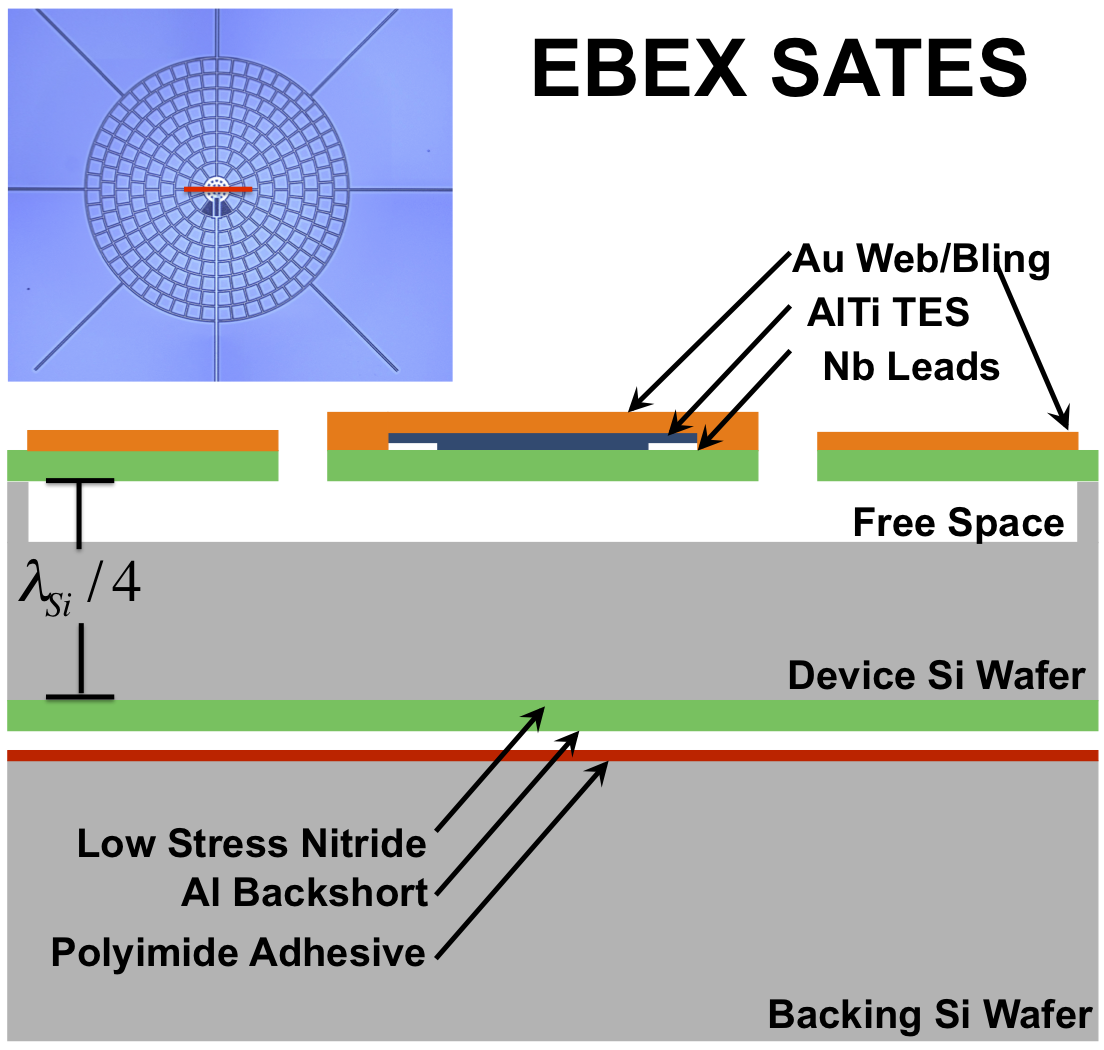
\includegraphics[width=0.68\textwidth]{./images/EBEX_Fab_Stack.pdf}\label{subfig:Fab_Stack}}
\caption{A cross-sectional diagram of the layers of the \ac{EBEX} detectors through the red line shown in the photograph.  In order to maximize absorptivity across a given band the device silicon wafer thickness is chosen to be $\lambda_\mathrm{Si} /4$.}
\label{fig:EBEX_Fab_Stack}
\end{figure}



%------------------------------------------------
%\include{DetectorReadoutBibliography}
\end{document}